\section{Validation and Error Analysis}
\label{sec:validation}
\begin{sloppypar}
The comparisons with the rigid body in \cref{sec:results} already test the spring model. Here we check the solvers themselves.
The numbers are computed by the script \code{plot_validation.py} in \code{src/sim/}.
\end{sloppypar}

\subsection{Exact solution}
\label{sec:analytic}
Euler's equations have an exact solution in Jacobi elliptic functions \cite{landau}.
The spin about the middle axis is proportional to $\operatorname{sn}$, which changes sign every half period, so the body flips every $T/2$ with
\begin{equation}
\begin{aligned}
    T &= 4K(k)\sqrt{\tfrac{I_1I_2I_3}{(I_3-I_2)(L^2-2EI_1)}},\\
    k^2 &= \tfrac{(I_2-I_1)(2EI_3-L^2)}{(I_3-I_2)(L^2-2EI_1)},
\end{aligned}
    \label{eq:jacobi-period}
\end{equation}
in Landau's labelling $I_1<I_2<I_3$, and $K$ the complete elliptic integral of the first kind.
\begin{sloppypar} % function names would otherwise stick out of the column
For the main run $1-k^2=4.9\times10^{-6}$; this close to the separatrix $1-k^2$ has to be computed directly, not as 1 minus $k^2$, or most of its digits are lost.
The solution, evaluated with \code{scipy.special.ellipj} and \code{ellipkm1} \cite{scipy}, gives flips every $T/2=\SI{31.213}{s}$, the same times as in \cref{tab:flips}.
The simulated $\vb*{\Omega}$ differs from it by a median of $2\times10^{-4}\,\si{rad/s}$, mostly from the finite-difference velocities.
\end{sloppypar}

\subsection{Conservation and convergence}
\label{sec:conservation}
\Cref{fig:conservation} follows the energy and angular momentum over \SI{100}{s}.
With velocity Verlet the energy error stays bounded, $2.5\times10^{-7}$ at $\Delta t=\SI{1}{ms}$ and four times smaller at half the step, and $\vb{L}$ is conserved to round-off, $3\times10^{-14}$, because the spring forces are central.
With RK4 the error is not bounded and builds up at each flip, but it is still only $8\times10^{-10}$ after \SI{100}{s} at $\Delta t=\SI{50}{ms}$.

\Cref{fig:convergence} confirms the order of both methods: $p=4.00$ for RK4 and $p\to2.00$ for Verlet.
Verlet only reaches its order once $\Delta t$ resolves the spring vibrations, 160--\SI{775}{rad/s}.
With the larger steps used in practice the phase of these vibrations is lost and the position error stays at a few $\si{\micro m}$, while the slow rotation that we measure stays accurate.

\begin{figure}[htb]
    \centering
    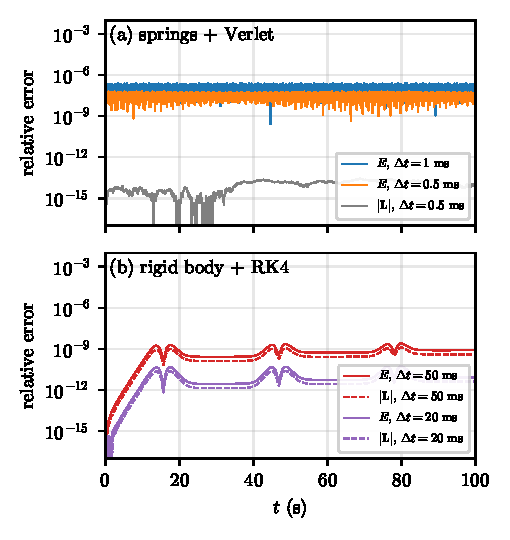
\includegraphics[width=\linewidth]{Images/conservation.pdf}
    \caption{Relative change of the energy and angular momentum. (a) Spring engine with Verlet. (b) Rigid-body solver with RK4.}
    \label{fig:conservation}
\end{figure}

\begin{figure}[htb]
    \centering
    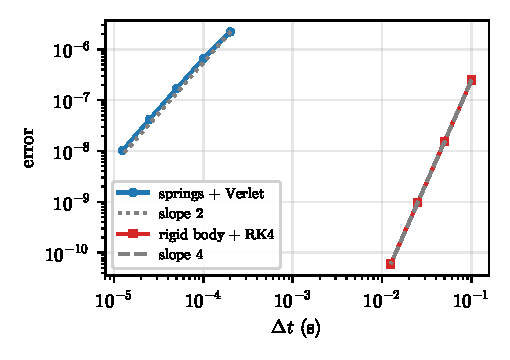
\includegraphics[width=\linewidth]{Images/convergence.pdf}
    \caption{Error against time step: Verlet (positions after \SI{1}{s}) and RK4 ($\vb*{\Omega}$ and $q$ after \SI{10}{s}), with slopes 2 and 4.}
    \label{fig:convergence}
\end{figure}

\subsection{Error budget}
\label{sec:error-budget}
The Python and Rust engines give bit-for-bit identical results after $10^5$ steps, and the stiffness error of the growth rate in \cref{tab:lambda} falls as about $(\SI{1.2}{N/m})/k$.
\Cref{tab:error-budget} collects the error sources for the main run.
The largest is not in the simulation but in the analysis, which reconstructs velocities from positions saved at \SI{60}{Hz}.

\begin{table}[htb]
    \centering
    \caption{Error sources for the main run ($\Delta t=\SI{e-5}{s}$, $k=\SI{e5}{N/m}$).}
    \label{tab:error-budget}
    \small
    \begin{tabular}{@{}lc@{}}
        \toprule
        Source & Relative size \\
        \midrule
        Time step (energy error)     & $\sim10^{-11}$ \\
        Finite stiffness ($\lambda$) & $\sim10^{-5}$ \\
        Velocities from \SI{60}{Hz} output & $\sim10^{-4}$ \\
        Floating point               & $\sim10^{-14}$ \\
        \bottomrule
    \end{tabular}
\end{table}
